%% Adaptado a partir de :
%%    abtex2-modelo-trabalho-academico.tex, v-1.9.2 laurocesar
%% para ser um modelo para os trabalhos no IFSP-SPO

\documentclass[
    % -- opções da classe memoir --
    12pt,               % tamanho da fonte
    openright,          % capítulos começam em pág ímpar (insere página vazia caso preciso)
    %twoside,            % para impressão em verso e anverso. Oposto a oneside
    oneside,
    a4paper,            % tamanho do papel. 
    % -- opções da classe abntex2 --
    %chapter=TITLE,     % títulos de capítulos convertidos em letras maiúsculas
    %section=TITLE,     % títulos de seções convertidos em letras maiúsculas
    %subsection=TITLE,  % títulos de subseções convertidos em letras maiúsculas
    %subsubsection=TITLE,% títulos de subsubseções convertidos em letras maiúsculas
    % Opções que não devem ser utilizadas na versão final do documento
    %draft,              % para compilar mais rápido, remover na versão final
    MODELO,             % indica que é um documento modelo então precisa dos geradores de texto
    TODO,               % indica que deve apresentar lista de pendencias 
    % -- opções do pacote babel --
    english,            % idioma adicional para hifenização
    brazil              % o último idioma é o principal do documento
    ]{ifsp-spo-inf-ctds}

        
% ---

% --- 
% CONFIGURAÇÕES DE PACOTES
% --- 
%\usepackage{etoolbox}
%\patchcmd{\thebibliography}{\chapter*}{\section*}{}{}


% ---
% Informações de dados para CAPA e FOLHA DE ROSTO
% ---
\titulo{SCRUM}

% Trabalho individual
\autor{JOSÉ BRAZ DE ARAUJO}

% Trabalho em Equipe
% ver também https://github.com/abntex/abntex2/wiki/FAQ#como-adicionar-mais-de-um-autor-ao-meu-projeto
%\renewcommand{\imprimirautor}{
%\begin{tabular}{lr}
%Aluno 1  & prontuario1 \\
%ALUNO 2 com sobrenome grande & prontuario2 \\
%ALUNO 3 & prontuario3 \\
%ALUNO 4 & prontuario4 \\
%\end{tabular}
%}


\tipotrabalho{Projeto da Disciplina XXXX}

\disciplina{XXXXX - Nome da Disciplina}

\preambulo{Proposta de projeto para disciplina XXXX}

\data{DATA DO TRABALHO}

% Definir o que for necessário e comentar o que não for necessário
% Utilizar o Nome Completo, abntex tem orientador e coorientador
% então vão ser utilizados na definição de professor
\renewcommand{\orientadorname}{Professor:}
\orientador{NOME COMPLETO DO PROFESSOR1}
\renewcommand{\coorientadorname}{Professor:}
\coorientador{NOME COMPLETO DO PROFESSOR2}



% ---


% ---
% Configurações de aparência do PDF final


% informações do PDF
\makeatletter
\hypersetup{
        %pagebackref=true,
        pdftitle={\@title}, 
        pdfauthor={\@author},
        pdfsubject={\imprimirpreambulo},
        pdfcreator={LaTeX with abnTeX2},
        pdfkeywords={abnt}{latex}{abntex}{abntex2}{trabalho acadêmico}, 
        colorlinks=true,            % false: boxed links; true: colored links
        linkcolor=blue,             % color of internal links
        citecolor=blue,             % color of links to bibliography
        filecolor=magenta,              % color of file links
        urlcolor=blue,
        bookmarksdepth=4
}
\makeatother
% --- 

% ---

% ----
% Início do documento
% ----
\begin{document}

% Retira espaço extra obsoleto entre as frases.
\frenchspacing 

\pretextual

% ---
% Capa - Para proposta a folha de rosto é suficiente pois é mais completa.
% ---
\imprimirfolhaderosto
% ---

% ----------------------------------------------------------
% ELEMENTOS TEXTUAIS
% ----------------------------------------------------------
\textual

\chapter[Introdução]{Introdução}
    
    Dados do IBGE apontam que de 2013 a 2020 ocorreu aumento da população de animais de estimação (cães, gatos, aves e répteis) nos domicílios brasileiros, como mostra o gráfico da figura \ref{fig:grafico pet}, ainda que a quantidade de domicílios com animais tenha sofrido uma pequena queda \cite{ibge2013} \cite{pet2021}, o mercado pet no Brasil encontra-se em ascensão nos últimos anos.
    
    Ainda de acordo com o instituto, aproximadamente 45\% dos lares possuem algum cão, e 19\% possuem algum gato,\cite{cao2019,} \cite{gato2019} movimentando cerca de R\$5 bilhões de reais entre 2020-2021 apenas com serviços e produtos veterinários, não contabilizando as outras subáreas do mercado pet, que movimentaram, no total, R\$ 45 bilhões de reais durante o mesmo biênio \cite{pet2021}.
    
    Dados do censo do Programa Nacional de Saúde mostram que, dos domicílios em que exitem um cão ou gato, 72\% vacinaram seus animais contra a raiva \cite{vacina2019}. Esse dado sugere que mais da metade dos tutores se preocupam com a saúde dos seus animais e procuram o profissional médico veterinário para garantir a profilaxia \cite{vacina2019}.
     
    Observando tais dados referentes ao censo populacional de cães e gatos no país, é esperado que estabelecimentos veterinários estejam sujeitos a rigorosas leis e fiscalização por parte dos seus órgãos de classe e sanitários.
    
    O CFMV (Conselho Federal de Medicina Veterinária), responsável por fiscalizar, orientar, supervisionar e disciplinar o exercício profissional de médicos veterinários e zootecnistas em âmbito federal, e os CRMVs (Conselho Regional de Medicina Veterinária) que tem como principal escopo a fiscalização do exercício das profissões das áreas de medicina veterinária e de zootecnia, de extensão regional\cite{doc_obrig} têm a competência para fiscalizar a aderência das clínicas e profissionais às normas éticas e de  operacionais.
     
    Dentre as responsabilidades dos profissionais médicos veterinários esta a emissão de documentos obrigatórios que comprovem o estado de saúde dos animais atendidos, dados de identificação desse animal, procedimentos realizados, medicações utilizadas, assim como resultados de exames, laudos, emissão de documentos complementares ou quaisquer outros dados relevantes.
    
    Ainda como responsabilidade do médico, é necessário que os documentos sejam armazenados por um prazo pré-definido de 2 a 20 anos. Estes documentos são utilizados pelas unidades fiscalizadoras quando requisitados, em fins jurídicos em caso de processos, assim como devem estar disponíveis para o tutor do animal \cite{doc_obrig}.
     
     \begin{figure}[H]
        \centering
        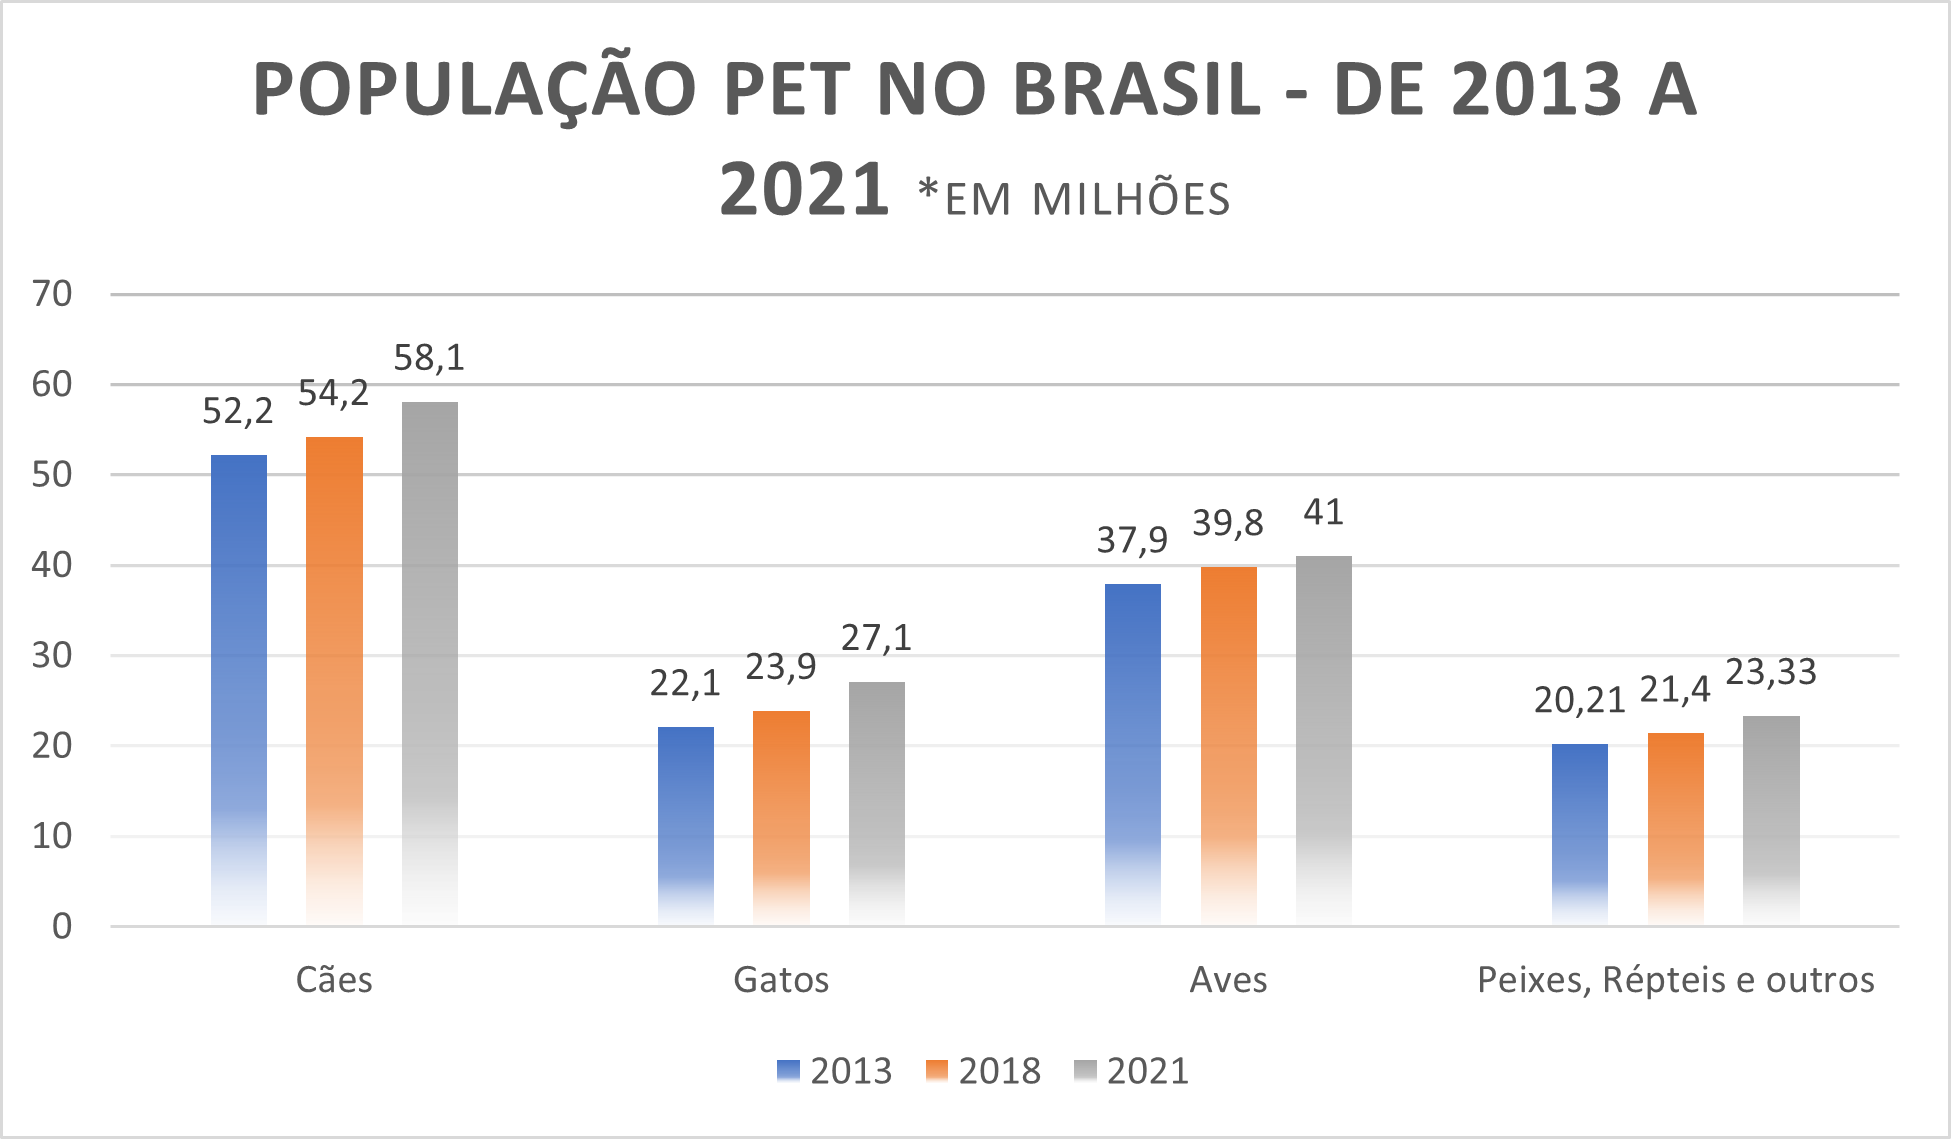
\includegraphics{images/grafico_censopet.png}
        \caption{Censo população Pet no Brasil\cite{ibge2013, ibge2018, pet2021}}
        \label{fig:grafico pet}
    \end{figure}

    \section{Análise da situação atual}
    
    O documento obrigatório de maior valor durante o atendimento é, sem dúvidas, o prontuário veterinário. Atualmente são utilizados tanto versões físicas como versões digitais, ou eletrônicas, dos prontuários.
    
    Os prontuários eletrônicos são oferecidos por diversos sistemas de gerenciamento de clínicas veterinárias, sendo amplamente empregados por oferecerem armazenamento com acesso fácil aos dados dos prontuários. Apesar da fidelidade das versões virtuais, os dados armazenados não podem substituir documentos físicos em eventos judiciais por não serem devidamente disciplinados por órgão regulamentador, nesse caso, pelos órgãos de classe que atestem a validade \cite{pe_dig} \cite{prontuario}.

    Além da questão regulatória, os sistemas de prontuários digitais atualmente disponíveis no mercado não torna os documentos imutáveis ou registram histórico de modificações. Assim, ao permitirem a alteração dos dados inseridos, não permitirem consultar o histórico de alterações ou meios de rastreá-las, sujeita o estabelecimento ao risco desamparo em caso de fiscalização por órgãos públicos ou perícias judiciais.
    
    Haja vista a falta de dificuldade dos sistemas atuais de dar apoio em caso de fiscalizações e a premissa da existência de arquivos físicos, torna-se necessário manter os registros físicos em pastas-fichários após serem carimbados e assinados pelo médico veterinário \cite{pe_dig}.
    
    O gerenciamento dos medicamentos controlados é realizado através de anotações manuais em um livro de registro. Esses registros devem ser realizadas periodicamente e com exatidão pelo profissional veterinário, orientando e definindo os procedimentos a serem adotados dentro da clínica, a fim de prevenir descumprimentos das orientações. No entanto, demandam reserva de tempo e atenção para a execução de alguns desses procedimentos, como a operação de cálculos manuais para cada valor ou a repetição de anotações de mesmos dados em diferentes documentos, podendo interferir na performance e exigindo mais esforço do profissional \cite{normativa}.
    
    Além das desvantagens supracitadas, o armazenamento desses arquivos ocupa espaço físico e estão sujeitos a danos e perdas por mau armazenamento, como incidentes gerados por umidade, fogo, roubos e etc. O preenchimento desses dados em versões físicas e depois transcritos para versões digitais, pode ser um processo demorado e é sujeito a falhas, demandando um tempo que poderia ser melhor aplicado pelos profissionais envolvidos. Além disso, torna-se necessário um grau elevado de organização por parte da clínica, de tal modo que não prejudique que a consulta aos arquivos seja possível de forma a facilitar o serviço do profissional\cite{pe_dig}.

    \section{Objetivos}

    A área de medicina veterinária ainda hoje opera de forma conservadora devido às suas necessidades burocráticas. E, por mais que o mercado ofereça algumas aplicações que têm a finalidade de automatizar o serviço, é difícil encontrar uma opção que ofereça funcionalidades que cumpram completamente as necessidades dos profissionais. Um dos motivos é que as soluções não são focadas em procedimentos específicos da veterinária, dividindo o ferramenta da aplicação com a gestão de Pet Shop.
    
    A aplicação, chamada de CertVet, tem como objetivo cobrir as principais necessidades de atuação do médico veterinário, automatizando os processos operacionais de atendimento e documentações clínicas, que hoje ainda demandam esforços manuais, cumprimento de normas legais e regulamentares e proponha um fluxo do trabalho eficiente, diminuindo o tempo gasto neste, a fim de melhorar o desempenho do profissional, do atendimento e consequentemente da clínica.


    \section{Justificativa}

    Assim como o número de animais de companhia cresce a cada ano, a quantidade de profissionais veterinários atuantes no mercado brasileiro também apresenta crescimento, com 164.549 médicos veterinários inscritos de acordo com a contabilização do órgão federal, indicado na figura \ref{fig:grafico vet} \cite{vets_SP, vets2020, vets2022}.
    
    \begin{figure}[H]
        \centering
        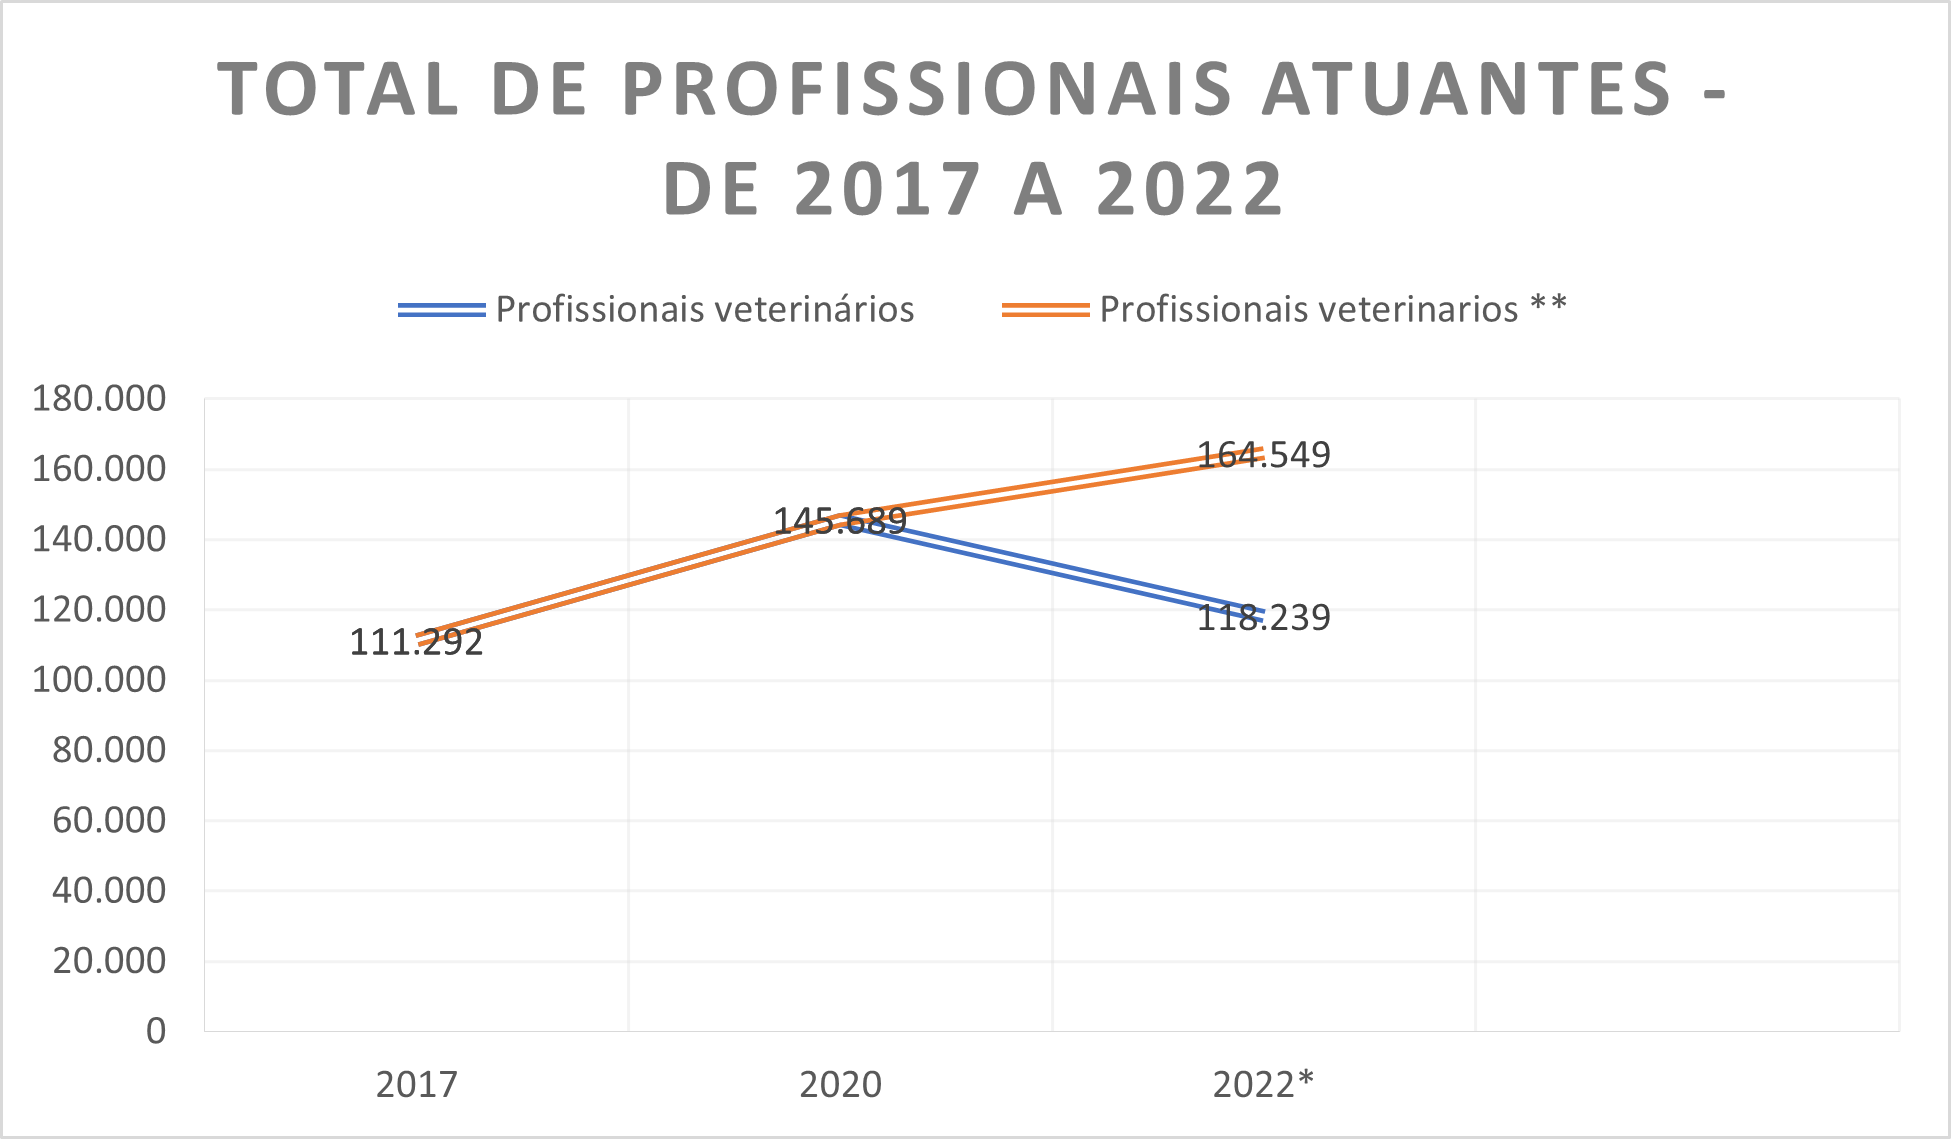
\includegraphics{images/grafico_profissionais.png}
        \caption{*Dados sem contabilizar os inscritos em SP; ** dados incluindo os inscritos em SP\cite{vets2020,vets2022} }
        \label{fig:grafico vet}
    \end{figure}
    
    De acordo com o último censo divulgado pelo CFMV (biênio 2021/2022), atualmente existem 46.947 registros ativos de estabelecimentos veterinários, sendo divididos entre clínicas, hospitais, consultórios e ambulatórios, como podemos ver na figura \ref{fig:grafico clinicas} \cite{clinicas2022}
    
    \begin{figure}[H]
        \centering
        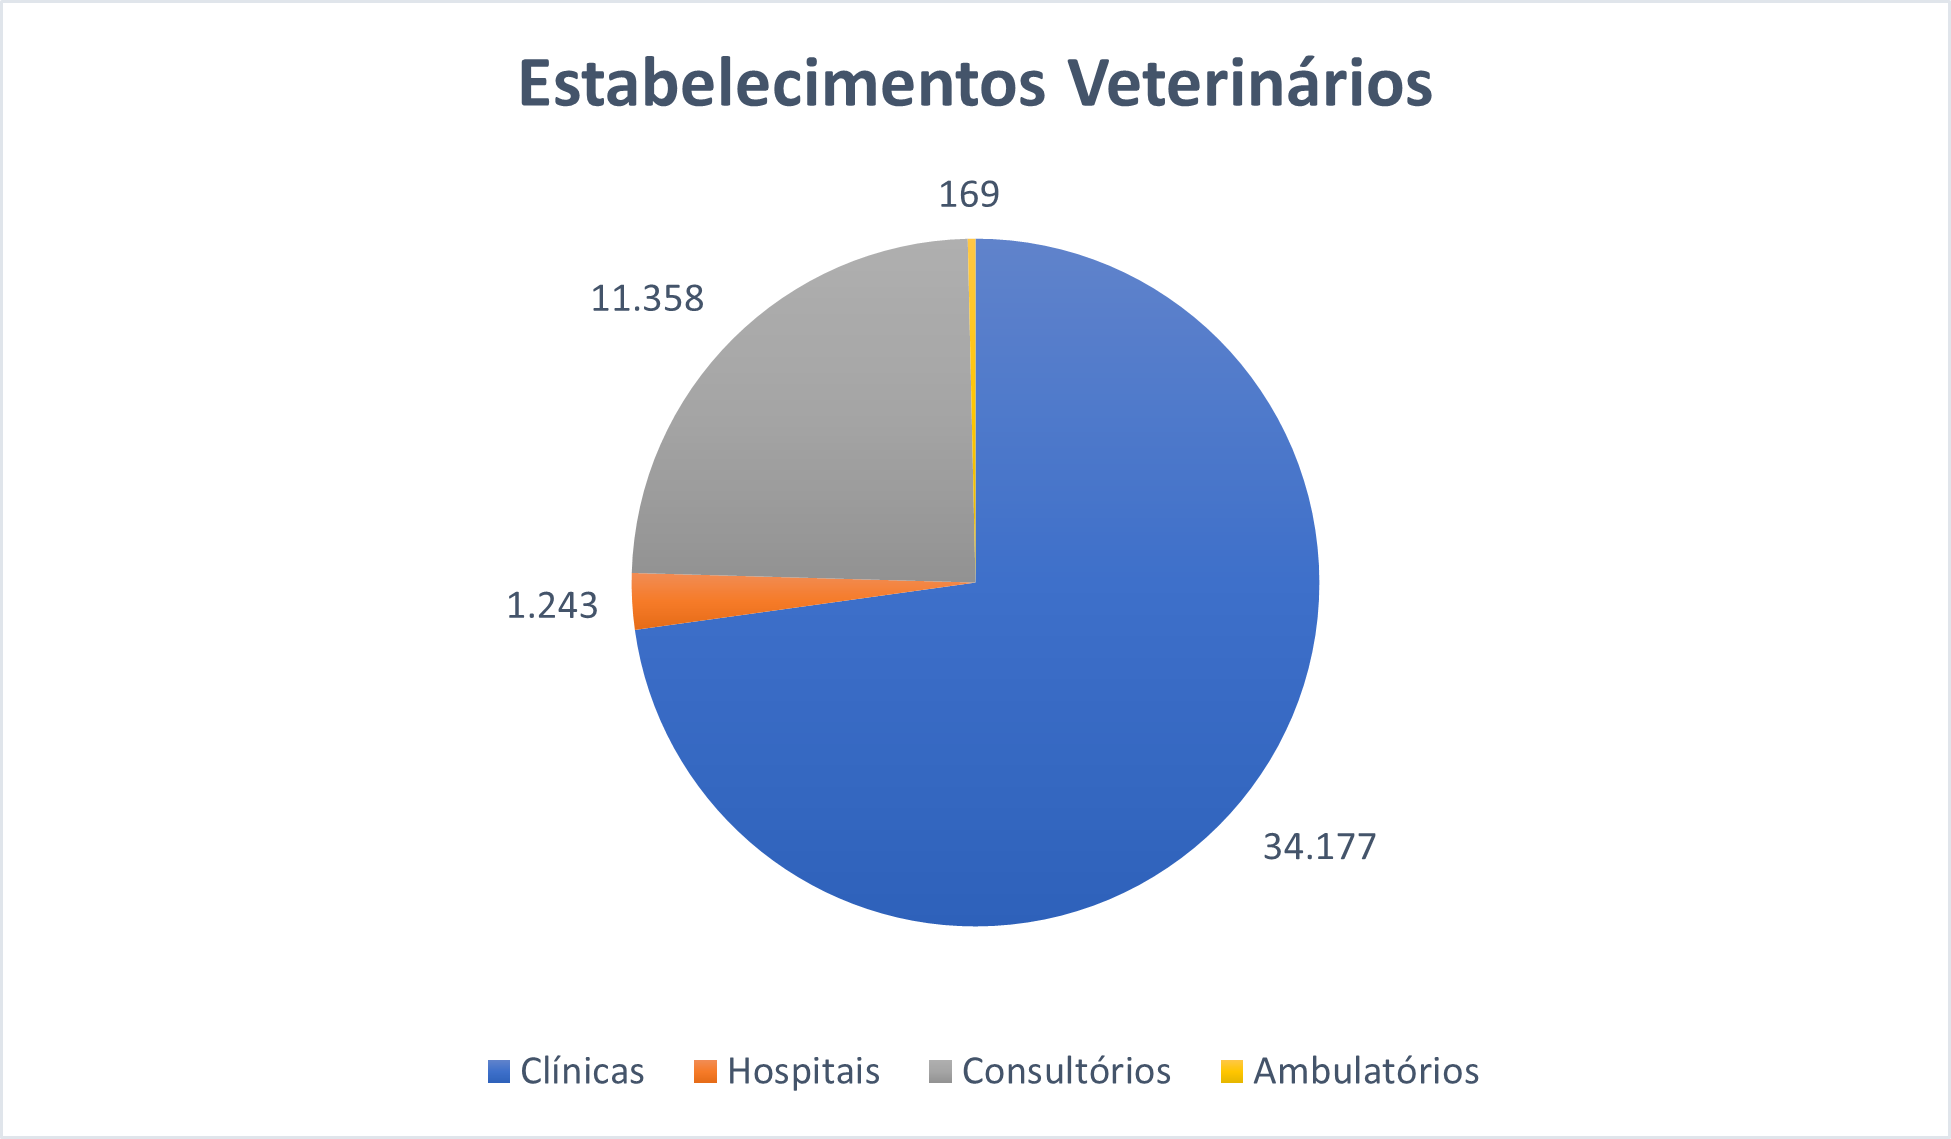
\includegraphics{images/grafico_estabelecimento.png}
        \caption{Censo estabelecimentos veterinários no biênio 2021/2022\cite{clinicas2022}}
        \label{fig:grafico clinicas}
    \end{figure}
    
    Todos esses profissionais e estabelecimentos são fiscalizados e disciplinado pelas regras de conduta dos sistemas CFMV/CRMVs.
    
    Visando oferecer funcionalidades que permitam uma dinamização de todo o fluxo de trabalho do profissional veterinário, reduzir o tempo gasto com operações manuais, evitar a necessidades de anotações de informações repetidamente e reduzir o risco de erros de transcrição nas documentações, a CertVet consiste em um sistema que gerencia documentos com potencial valor legal e seus processos processos que se fazem necessários no fluxo de trabalho da medicina veterinária.
    
    Os processos automatizados agilizam os procedimentos fiscalizatórios e permitem que as alterações feitas sejam rastreadas, como é exigida pelo CFMV (Conselho Federal de Medicina Veterinária) e pelo CRMVs (Conselho Regional de Medicina Veterinária)\cite{teleMV}.
    
    A tecnologia da informação está modernizando a rotina de trabalho em áreas como automações de escritório, farmacêuticas e na medicina humana em estágios bem mais avançados que em relação ao atualmente aplicado na medicina veterinária. Entendemos que existe a oportunidade de propor ritmo mais acelerado sem impedir a legalidade dos processos dentro de uma clínica veterinária.
    
    A partir das verificações de ambiente, referencial regulatório e constatação da situação, verificamos que o desenvolvimento de uma aplicação focada na automação de processos operacionais que otimizando o tempo de execução das tarefas do profissional veterinário e confiabilidade dos registros inseridos.
    
    Em pesquisa bibliográfica, não foram identificados fatos referentes a quantidade de profissionais ou estabelecimentos que utilizam algum sistema eletrônico ou de gestão. Porém, os meios de comunicação comumente enfatizam o crescimento de relevância econômica de serviços para o mercado de animais de estimação ano a ano. O sistema CertVet tem potencial para crescer e se destacar entre os demais sistemas já existentes.
    
    \chapter{Revisão da Literatura}

    Este capítulo abordará uma breve revisão bibliográfica sobre a documentação obrigatória emitida por estabelecimentos veterinários, revisão das leis referentes a tais documentos, novos caminhos abordados pelo Conselho Federal de Medicina Veterinária e como esse aspectos são relevantes ao nosso projeto.


    \section{Documentação Obrigatória e Legislação Pertinente}
    
        De acordo com a Resolução nº1321, de 24 de abril de 2020 \cite {doc_obrig}, todo estabelecimento veterinário e/ou médico veterinário deve emitir documentos específicos no âmbito de suas respectivas atividades profissionais.
        
        Tais documentos, de caráter obrigatório, deve seguir os padrões estabelecidos pelo Conselho Federal de Medicina Veterinária, que regulamenta a profissão do médico veterinário, de acordo com a Lei nº 5.517, alínea “f”, do artigo 16, de 23 de outubro de 1968. \cite {doc_obrig}.
        
        A Resolução 1321/2020, em seu Art. 2º, define o prontuário veterinário como \cite {doc_obrig}: 
    
        \begin{quote}
            VIII - prontuário médico-veterinário: documento escrito e datado, sem rasuras ou emendas, emitido e assinado, privativamente por médico-veterinário que relata e detalha, cronologicamente, informações e dados acerca dos atendimentos ambulatoriais e clínicos, inclusive vacinações, exames diagnósticos e intervenções cirúrgicas realizados em animal, ou coletivo em se tratando de rebanho, garantida a autenticidade e integridade das informações;
        \end{quote}
    
        Outros documentos obrigatórios são \cite{doc_obrig}.: 
    
        \begin{itemize}
            \item
            Atestado ou declaração de óbito,
            \item
            Atestado ou declaração de vacinação,
            \item
            Atestado sanitário,
            \item
            Prontuário médico-veterinário,
            \item
            Termo de consentimento livre esclarecido para realização de exames, 
            \item
            Termo de consentimento livre esclarecido para realização de procedimentos terapêuticos de risco ou experimental, 
            \item
            Termo de consentimento livre esclarecido para retirada de corpo de animal em óbito, 
            \item
            Termo de consentimento livre esclarecido para realização de procedimento cirúrgico, 
            \item
            Termo de consentimento livre esclarecido para realização de procedimento anestésico, 
            \item
            Termo de consentimento livre esclarecido para internação e tratamento clínico ou pós-cirúrgico, 
            \item
            Termo de consentimento livre esclarecido para realização de eutanásia, 
            \item
            Termo de consentimento livre esclarecido para retirada do serviço veterinário sem alta médica, 
            \item
            Termo de consentimento livre esclarecido para doação de corpo de animal para ensino e pesquisa, 
            \item
            Termo de consentimento livre esclarecido para realização de pesquisa clínica.
        \end{itemize}
    
        Dentre as regras referidas na resolução nº 1321 de 2020, seu artigo 3º disciplina dados para a composição do prontuário médico:
    
        \begin{quote}
            Os documentos emitidos por médicos-veterinários comporão o prontuário do paciente (...) conter os seguintes dados e informações: nome completo e assinatura do médico-veterinário, número de inscrição no Sistema CFMV/CRMVs, endereço, telefone, e-mail e, se for o caso, identificação do estabelecimento (razão social, CNPJ e número de registro no Sistema CFMV/CRMVs)
        \end{quote}
    
        No inciso VI, especifica fatos relacionados ao animais que devem constar por observação física:
        
        \begin{quote}
            (Deve) conter informações que permitam a identificação do paciente, tais como nome, sexo, raça, idade real ou presumida, cor de pelagem ou plumagem, sinais particulares, tatuagem, brinco, microchip, registro genealógico e, conforme o caso, resenha detalhada;(...) identificação do responsável pelo animal (nome completo, CPF e endereço completo)
        \end{quote}
    
        Em seu inciso VII, § 2º, dispõe sobre requisitos para operação de através de mídias virtuais: 
    
        \begin{quote}
            Os documentos expedidos eletronicamente deverão contar com sistemas capazes de garantir a segurança, autenticidade, confidencialidade e integridade de informações, bem como o armazenamento e compartilhamento dos dados.
        \end{quote}
    
        Tais regulamentações garantem a legitimidade do sistema proposto pela equipe Rocket, sendo embasamento legal e diretrizes a serem seguidas.
        
        A autorização para se realizar a telemedicina na área veterinária também adere à tendência de modernização na profissão e viabiliza que soluções digitais sejam implementadas relativas a documentação obrigatória.\cite{teleMV}.
        
        Com relação a gestão de medicamentos controlados (de uso restrito e com retenção de receitas), de acordo com as leis vigentes da INSTRUÇÃO NORMATIVA Nº 35, DE 11 DE SETEMBRO DE 2017, Capítulo I, Art. 2º, § IV, Capitulo IV, § 11  \cite{normativa}, ela é realizada através de um caderno de capa dura, no formato brochura, no qual o médico veterinário responsável técnico (RT) anota a data de entrada dos medicamentos no estoque e quanto desse medicamento foi utilizado no dia, para cada procedimento. Este caderno é denominado Livro-Registro.




        % dentro do capitulo 3- metodologias, seção 4.4

        \subsection{Histórias de Usuários}
    
    \begin{center}
        \begin{table}[H]
        \centering
        \begin{tabulary}{1.0\textwidth}{|p{5em}|p{8em}|p{18em}|}
        \hline
        Código & História & Descrição\\
        \hline
        HU-01 & Função gerar documento com assinatura digital/certificação & Eu como usuário autorizado, quero gerar um documento oficial com assinatura digital, que me permita rastrear todas suas versões anteriores, para que sejam rastreáveis e passíveis de identificação.\\
        \hline
        HU-02 & Função preencher prontuário & Eu como usuário autorizado, quero preencher um prontuário para um animal em atendimento, para que seus dados sejam salvos.\\
        \hline
        HU-03 & Função salvar prontuário & Eu como usuário autorizado, quero salvar o prontuário digital, para que seja possível sua leitura em momento posterior.\\
        \hline
        HU-04 & Função uso de medicamentos controlados & Eu como usuário autorizado, quero anotar os medicamentos controlados utilizados no atendimento, para que seja possível seu controle com os dados do estoque.\\
        \hline
        HU-05 & Função inserir medicamentos no estoque & Eu, como usuário autorizado, quero inserir no sistema a quantidade total de produtos no estoque, para que seja possível o controle de quantidade usada por atendimento, perdida e que ainda está disponível.\\
        \hline
        HU-06 & Função visualizar prontuários & Eu, como usuário autorizado, quero acessar os prontuários de determinado animal, para que seja possível acompanhar seu histórico ou quadro clínico.\\
        \hline
        HU-07 & Função salvar dados genealógicos &  Eu, como usuário autorizado, quero inserir dados sobre pais e descendentes (quando existentes), na ficha médica do animal, para que tais dados estejam disponíveis para consulta quando necessário.\\
        \hline
        HU-08 &  Função recuperar dados genealógico &  Eu, como usuário autorizado, quero consultar a árvore genealógica do animal (quando disponível), para obter informações úteis ao tratamento do mesmo.\\
        \hline
        HU-09 & Função inserir dados na agenda & Eu, como funcionário, quero inserir dados de um atendimento na agenda, para que os atendimentos futuros sejam planejados.\\
        \hline
        HU-10 & Função cadastrar cliente & Eu, como funcionário, quero cadastrar um cliente no sistema, para que seus dados estejam disponíveis para uso dentro da clínica\\
        \hline
        \end{tabulary}
        \caption{Historias de Usuário}
        \label{tab:hist_usuario}
        \end{table}
    \end{center}
% ----------------------------------------------------------
% Referências bibliográficas
% ----------------------------------------------------------
\bibliography{referencias,exemplos/abntex2-doc-abnt-6023}

\end{document}
